\section{Parallel loop dependencies with OpenMP \punkte{15}}

The sequential baseline in Listing~\ref{lst:recur_seq} computes the geometric recurrence
\mbox{$S_{n+1} = S_n\cdot\texttt{up}$} while storing every intermediate value in the array
\texttt{opt}.  This version is inherently schedule independent and serves as the reference for
both correctness and runtime.  The first parallel attempt (Listing~\ref{lst:recur_chunk}) keeps
the same arithmetic but splits the index range into contiguous chunks.  Each thread receives its
starting index, reconstructs the corresponding value through a single
\texttt{pow(up, start)} call, and then advances with repeated multiplications.  In OpenMP this is
implemented with \texttt{firstprivate(Sn)} so that every thread starts from the same scalar value;
no \texttt{lastprivate} is required because the final value is written in the shared 
\texttt{opt\_chunk} array.  The approach is fully schedule independent, because every thread owns
disjoint indices.

Listing~\ref{lst:recur_dyn} shows the second variant, where I experimented with a
\texttt{schedule(dynamic)} loop.  The idea was to keep using \texttt{firstprivate(Sn)} and
\texttt{lastprivate(Sn)} and to recompute the state only when a thread receives a non-contiguous
block.  The helper variables \texttt{Sn\_local} and \texttt{last\_i} were added precisely for
that purpose: whenever the assigned iteration is not the immediate successor of the previous one,
the code falls back to \texttt{Sn * pow(up, i)}.  Unfortunately this makes the loop depend on the
OpenMP scheduler.  With the default dynamic scheduler the runtime hands out extremely small
chunks, so the costly \texttt{pow} is executed almost every iteration.  As a consequence the
dynamic version violates the assignment requirement of being schedule independent and performs
worse than the serial baseline.

\lstinputlisting[
    language=C,
    numbers=left,
    caption={Sequential recurrence baseline},
    captionpos=b,
    label={lst:recur_seq},
    linerange={6-35},
    firstnumber=6
]{../Skeleton\_codes/loop-dependencies/recur_seq.c}

\lstinputlisting[
    language=C,
    numbers=left,
    caption={Chunk-based parallel recurrence},
    captionpos=b,
    label={lst:recur_chunk},
    linerange={21-37},
    firstnumber=21
]{../Skeleton\_codes/loop-dependencies/recur_omp.c}

\lstinputlisting[
    language=C,
    numbers=left,
    caption={Dynamic schedule with on-demand recomputation},
    captionpos=b,
    label={lst:recur_dyn},
    linerange={39-53},
    firstnumber=39
]{../Skeleton\_codes/loop-dependencies/recur_omp.c}

The scaling study (Figure~\ref{fig:recur_scaling}) confirms these observations.  The chunk-based
parallelisation reaches nearly linear speedup: the runtime drops from roughly $6.7\,$s on one
thread to $0.39\,$s on twenty threads.  The dynamic variant, on the other hand, keeps increasing
from $134\,$s (one thread) to $344\,$s (twenty threads), which is even slower than the serial
baseline at the far left of the plot.  The experiment therefore illustrates that the manual chunk
partitioning satisfies the “schedule independent’’ requirement of the assignment, whereas the
dynamic version is dominated by the repeated \texttt{pow} calls triggered by OpenMP’s fine-grained
work distribution.

\begin{figure}[H]
    \centering
    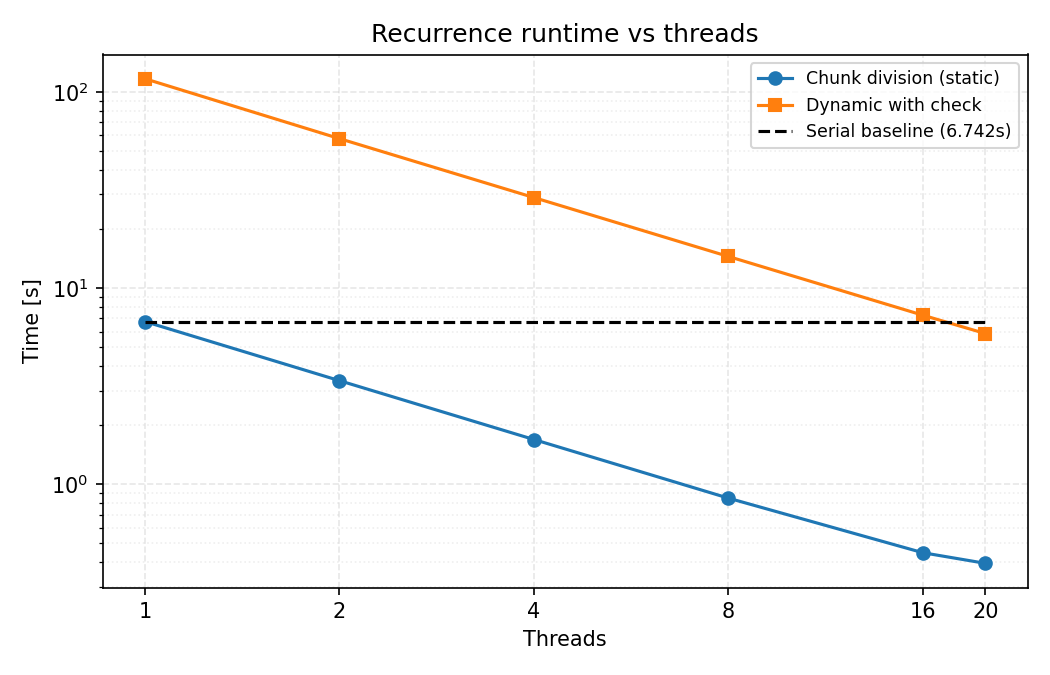
\includegraphics[width=0.75\linewidth]{../Skeleton\_codes/loop-dependencies/plots/recur_runtime_scaling.png}
    \caption{Runtime per thread count for the chunk and dynamic variants, compared with the serial baseline.}
    \label{fig:recur_scaling}
\end{figure}
